\documentclass[]{article}
\usepackage{tikz}
\usetikzlibrary{arrows,positioning,shapes,fit,calc}
\begin{document}
COMPOSITE FUNCTIONS\\
\begin{center}
    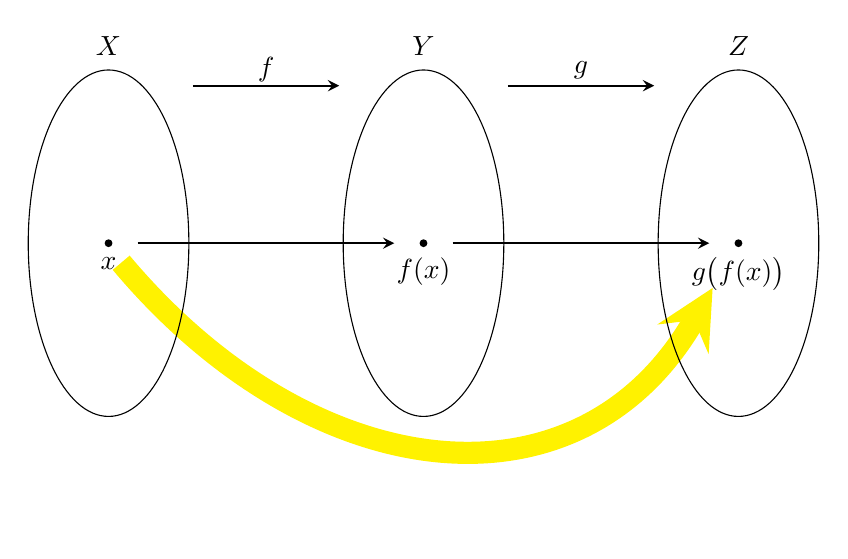
\begin{tikzpicture}[
    >=stealth,
    bullet/.style={
        fill=black,
        circle,
        minimum width=1pt,
        inner sep=1pt
    },
    projection/.style={
        ->,
        thick,
        shorten <=2pt,
        shorten >=2pt
    },
    every fit/.style={
        ellipse,
        draw,
        inner sep=0pt
    }
    ]
    \node at (2,4.7) {$f$};
    \draw[projection] (1,4.5) -- (3,4.5);
    \node at (0,5) {$X$};
    \node[bullet,label=below:$x$] (START)   at (0,2.5){};
    \node at (4,5) {$Y$};
    \node[bullet,label=below:$f(x)$] at (4,2.5){};
    \node at (6,4.7) {$g$};
    \draw[projection] (5,4.5) -- (7,4.5);
    \node at (8,5) {$Z$};
    \node[bullet,label=below:$g\big(f(x)\big)$] (END) at (8,2.5){};

    \draw [line width=8pt, yellow, shorten <=0.25cm,, shorten >=0.6cm, ->] (START.south) to[out=-50, in=-120, distance=4cm, ] (END);

    \draw (0,2.5) ellipse (1.02cm and 2.2cm);
    \draw (4,2.5) ellipse (1.02cm and 2.2cm);
    \draw (8,2.5) ellipse (1.02cm and 2.2cm);

    \draw[projection] (0.3,2.5) -- (3.7,2.5);
    \draw[projection] (4.3,2.5) -- (7.7,2.5);
    \end{tikzpicture}
    \newline
\end{center}
\end{document}